\chapter{Design and Implementation}
\label{cha:design}
\section{Toolchain}
\section{Board Configuration}
On the Hifive1, there are several important configuration options that affect general operation of the board. The most notable of these are the clock settings, as these indicate the frequency of the processor, input and output frequencies, and timer interrupts. 
\subsection{Clock settings}
% INCLUDE CLOCK USE FIGURE
The Hifive1 has 3 clock regions, a high frequency clock, a low frequency clock, and a clock used to drive the JTAG connection. The JTAG driver is constant and only used for debugging through JTAG, so is not relavent here.
\\

\begin{figure}[H]
    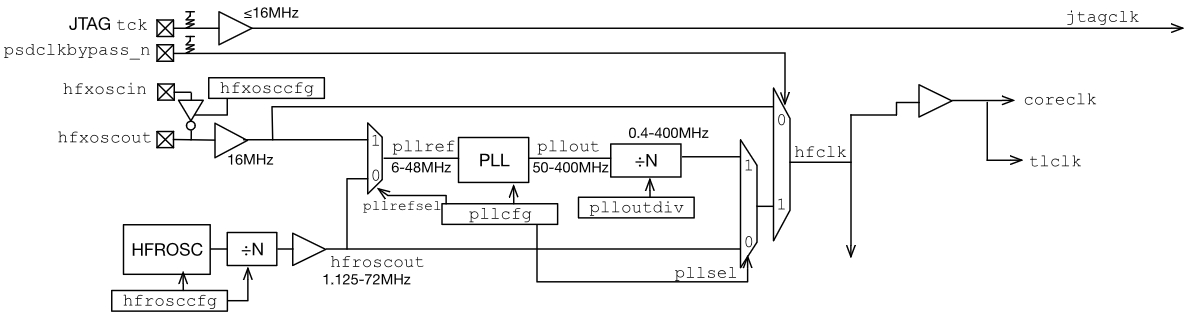
\includegraphics[width=0.9\columnwidth]{figures/hfclock.png}
    \caption[High Frequency Clock Diagram]{The high frequency clock generation scheme, specifying how the high frequency clock is driven and configured}
\end{figure}
The high frequency clock controls the processor frequency, and the baud rate of input and output is derived from it. The high frequency clock can be driven from two sources, an internally trimmable high frequency ring oscillator and an external high frequency crystal oscillator. The ring oscillator can produce frequencies ranging form ~1 MHz to 75 MHz, whereas the crytal will produce a constant frequency of 16 MHz. Both of these clock sources may be used `as is', or can be modified using a PLL and divider, giving a available range of 48 MHz to 384 MHz. 
\\
\begin{figure}[H]
    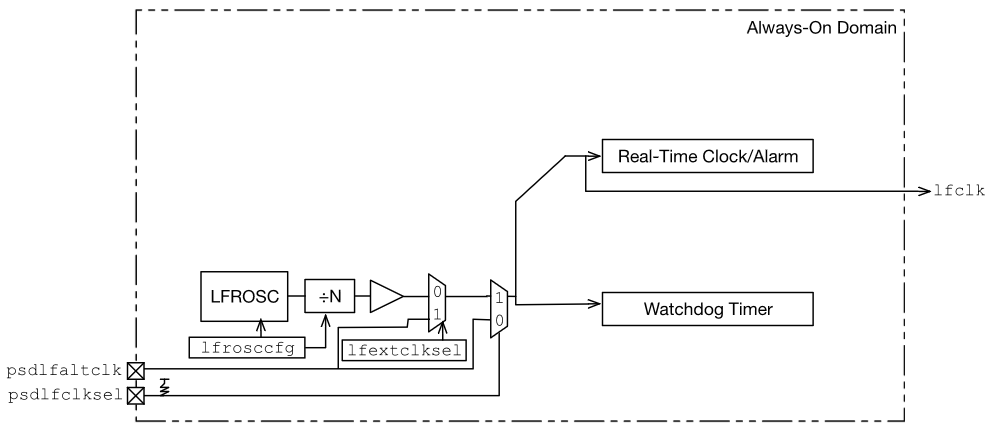
\includegraphics[width=0.9\columnwidth]{figures/lfclock.png}
    \caption[Low Frequency Clock Diagram]{The low frequency clock generation scheme, specifying how the low frequency clock is driven and configured}
\end{figure}
The low frequency clock is part of the Hifive1 `always on block' and controls the watchdog timer, which can be used to cause a reset on malfunction, and both the realtime clock and the machine timer, both of which are used to generate timed interrupts. Similar to the high frequency clock can be driven from a ring oscillator or from an external clock, which in the Hifive1 is a crystal oscillator. The low frequency ring oscillator functions at 1.5 KHz to 230 KHz using a frequency divider, and the implemented external clock runs at a contant 32.768 KHz, with no option to divide the frequency.
\\
For both clock domains, the crystal oscillator was chosen. The ring oscillator gives the option to operate at a higher frequency, which would result in a higher number of operations per second. While in a practical operating system this would be desirable, since this system is not intended for practical use, a constant frequency was more desirable as it would give more predictable results, and makes IO operations more reliable. For the low frequency clock, a high frequency would be beneficial for a real time system as the higher frequency would allow for more precise timing of interrupts and other functions, however for an interactive system this precision is not required, and so similar to the high frequency domain the constant frequency of a crystal oscillator was selected.
\section{Processes}
\section{Scheduler}
\section{Memory Management}
\section{IO}